\subsection{ViewModel}
\label{chap:viewmodel_design}
The \emph{view model} plays a crucial role in the architecture of an application. It serves as the intermediary between the \emph{view} and the \emph{model}.
The \emph{view model} is responsible for providing the necessary data and functionality to the \emph{view}, resulting in a clear separation between the \emph{view} and the \emph{model}.
By decoupling these components, the \emph{view model} supports separation of concerns.
In the system consists of three \emph{view models}, namely \emph{HrViewModel}, responsible for managing business logics related to heart rate and activity data, \emph{ExerciseViewModel}, which provides business logics for exercise related data, and lastly \emph{UserViewModel}, responsible for managing business logics related to user.

\subsubsection{HrViewModel}
As mentioned, the \emph{HrViewModel} is responsible for managing business logics related to the heart rate data and activity within the system.
This \emph{ViewModel} facilitates the communication between the \emph{HomeFragment} and the business logics related to the heart rate data and activity, for instance, \emph{connection service} and \emph{activity service}.
Additionally, it includes heart rate LiveData\footnote{\emph{LiveData} is an observable data holder class. LiveData follows the observable pattern and allows other components to observe changes in the data. URL: \url{https://developer.android.com/topic/libraries/architecture/livedata}} and activity LiveData, enabling the fragment to observe these data and receive updates whenever changes occur. This allows fragment to react accordingly and adjust the user interface correspondingly.
Furthermore, the \emph{HrViewModel} interacts with the repositories to perform necessary operations on heart rate data.
Sequence diagrams are created to visually represent the sequence of operations executed in \emph{HrViewModel}.

\begin{figure}[H]
    \centering
    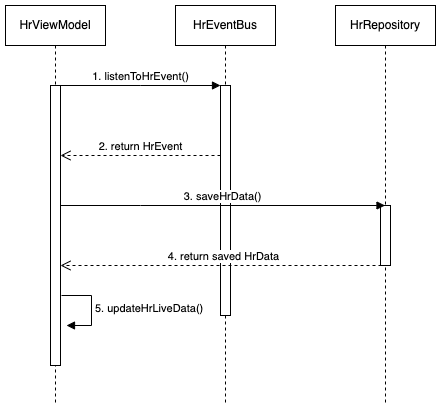
\includegraphics[width=0.7\textwidth]{diagrams/hrviewmodel-hr.drawio.png}
    \caption{HrViewModel heart rate data flow sequence diagram}
    \label{fig:hrviewmodel_hrdata}
\end{figure}

To provide the \emph{HomeFragment} with the actual heart rate data, the following sequence of operations is executed:
\begin{enumerate}
    \item The \emph{HrViewModel} actively listens to events published in \emph{HrEventBus}.
    \item Event containing heart rate data is retrieved.
    \item Heart rate from the event is extracted and sent to the repository to be persisted.
    \item Heart rate is saved in the database and returned to \emph{HrViewModel}
    \item \emph{HrViewModel} updates the heart rate LiveData.
\end{enumerate}

The following sequence of operations is executed to provide the \emph{HomeFragment} with up-to-date activity data.
\begin{enumerate}
    \item The \emph{HrViewModel} actively listens to events published in \emph{ActivityEventBus}.
    \item Event containing activity data is retrieved.
    \item \emph{HrViewModel} updates the activity LiveData.
\end{enumerate}

\begin{figure}[H]
    \centering
    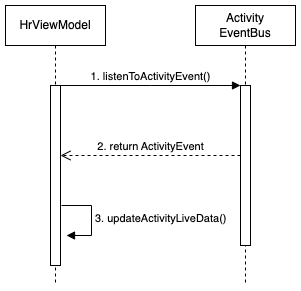
\includegraphics[width=0.5\textwidth]{diagrams/hrviewmodel-activity.drawio.png}
    \caption{HrViewModel activity data flow sequence diagram}
    \label{fig:hrviewmodel_activitydata}
\end{figure}

\subsubsection{ExerciseViewModel}
The \emph{ExerciseViewModel} is responsible for managing business logics related to exercise within the application.
It supports the communication between the \emph{ExerciseFragment} and the business logics related to exercise such as the \emph{ExerciseService}.
The \emph{ExerciseViewModel} also manages the current exercise LiveData, which holds the current exercise data and is observed by the \emph{ExerciseFragment} for real-time updates. 
Additionally, the ExerciseViewModel interacts with other components, for instance, the repositories to perform necessary operations to manage data.
To support the \emph{ExerciseFragment} with the actual exercise data, the following sequence of operations is provided.

\subsubsection{UserViewModel}
